% This file was created with tikzplotlib v0.10.1.
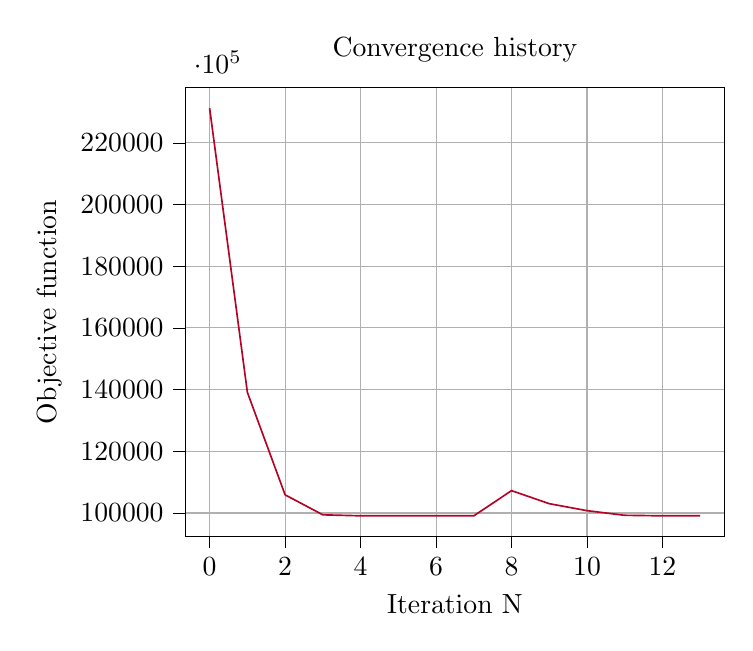
\begin{tikzpicture}

\definecolor{darkgray176}{RGB}{176,176,176}
\definecolor{firebrick180438}{RGB}{180,4,38}

\begin{axis}[
tick align=outside,
tick pos=left,
title={Convergence history},
x grid style={darkgray176},
xlabel={Iteration N},
xmajorgrids,
xmin=-0.65, xmax=13.65,
xtick style={color=black},
xtick={-2,0,2,4,6,8,10,12,14},
xticklabels={
  \(\displaystyle {\ensuremath{-}2}\),
  \(\displaystyle {0}\),
  \(\displaystyle {2}\),
  \(\displaystyle {4}\),
  \(\displaystyle {6}\),
  \(\displaystyle {8}\),
  \(\displaystyle {10}\),
  \(\displaystyle {12}\),
  \(\displaystyle {14}\)
},
y grid style={darkgray176},
ylabel={Objective function},
ymajorgrids,
ymin=92479.1845549044, ymax=237805.674215607,
ytick style={color=black},
ytick={80000,100000,120000,140000,160000,180000,200000,220000,240000},
yticklabels={
  \(\displaystyle {80000}\),
  \(\displaystyle {100000}\),
  \(\displaystyle {120000}\),
  \(\displaystyle {140000}\),
  \(\displaystyle {160000}\),
  \(\displaystyle {180000}\),
  \(\displaystyle {200000}\),
  \(\displaystyle {220000}\),
  \(\displaystyle {240000}\)
}
]
\addplot [semithick, firebrick180438]
table {%
0 231199.924685575
1 139115.71466262
2 105883.891802433
3 99406.9798995348
4 99085.9900030204
5 99084.934126946
6 99084.9341136118
7 99084.9341136118
8 107248.829074952
9 103020.371408933
10 100759.571286058
11 99250.5183147928
12 99084.9340849363
13 99084.9341136118
};
\end{axis}

\end{tikzpicture}
